%
% msa.tex -- visual representation of MSA
%
% (c) 2019 Prof Dr Andreas Müller, Hochschule Rapperswil
%
\documentclass[tikz]{standalone}
\usepackage{amsmath}
\usepackage{times}
\usepackage{txfonts}
\usepackage{pgfplots}
\usepackage{csvsimple}
\usetikzlibrary{arrows,intersections,math,fadings,shadings}
\begin{document}
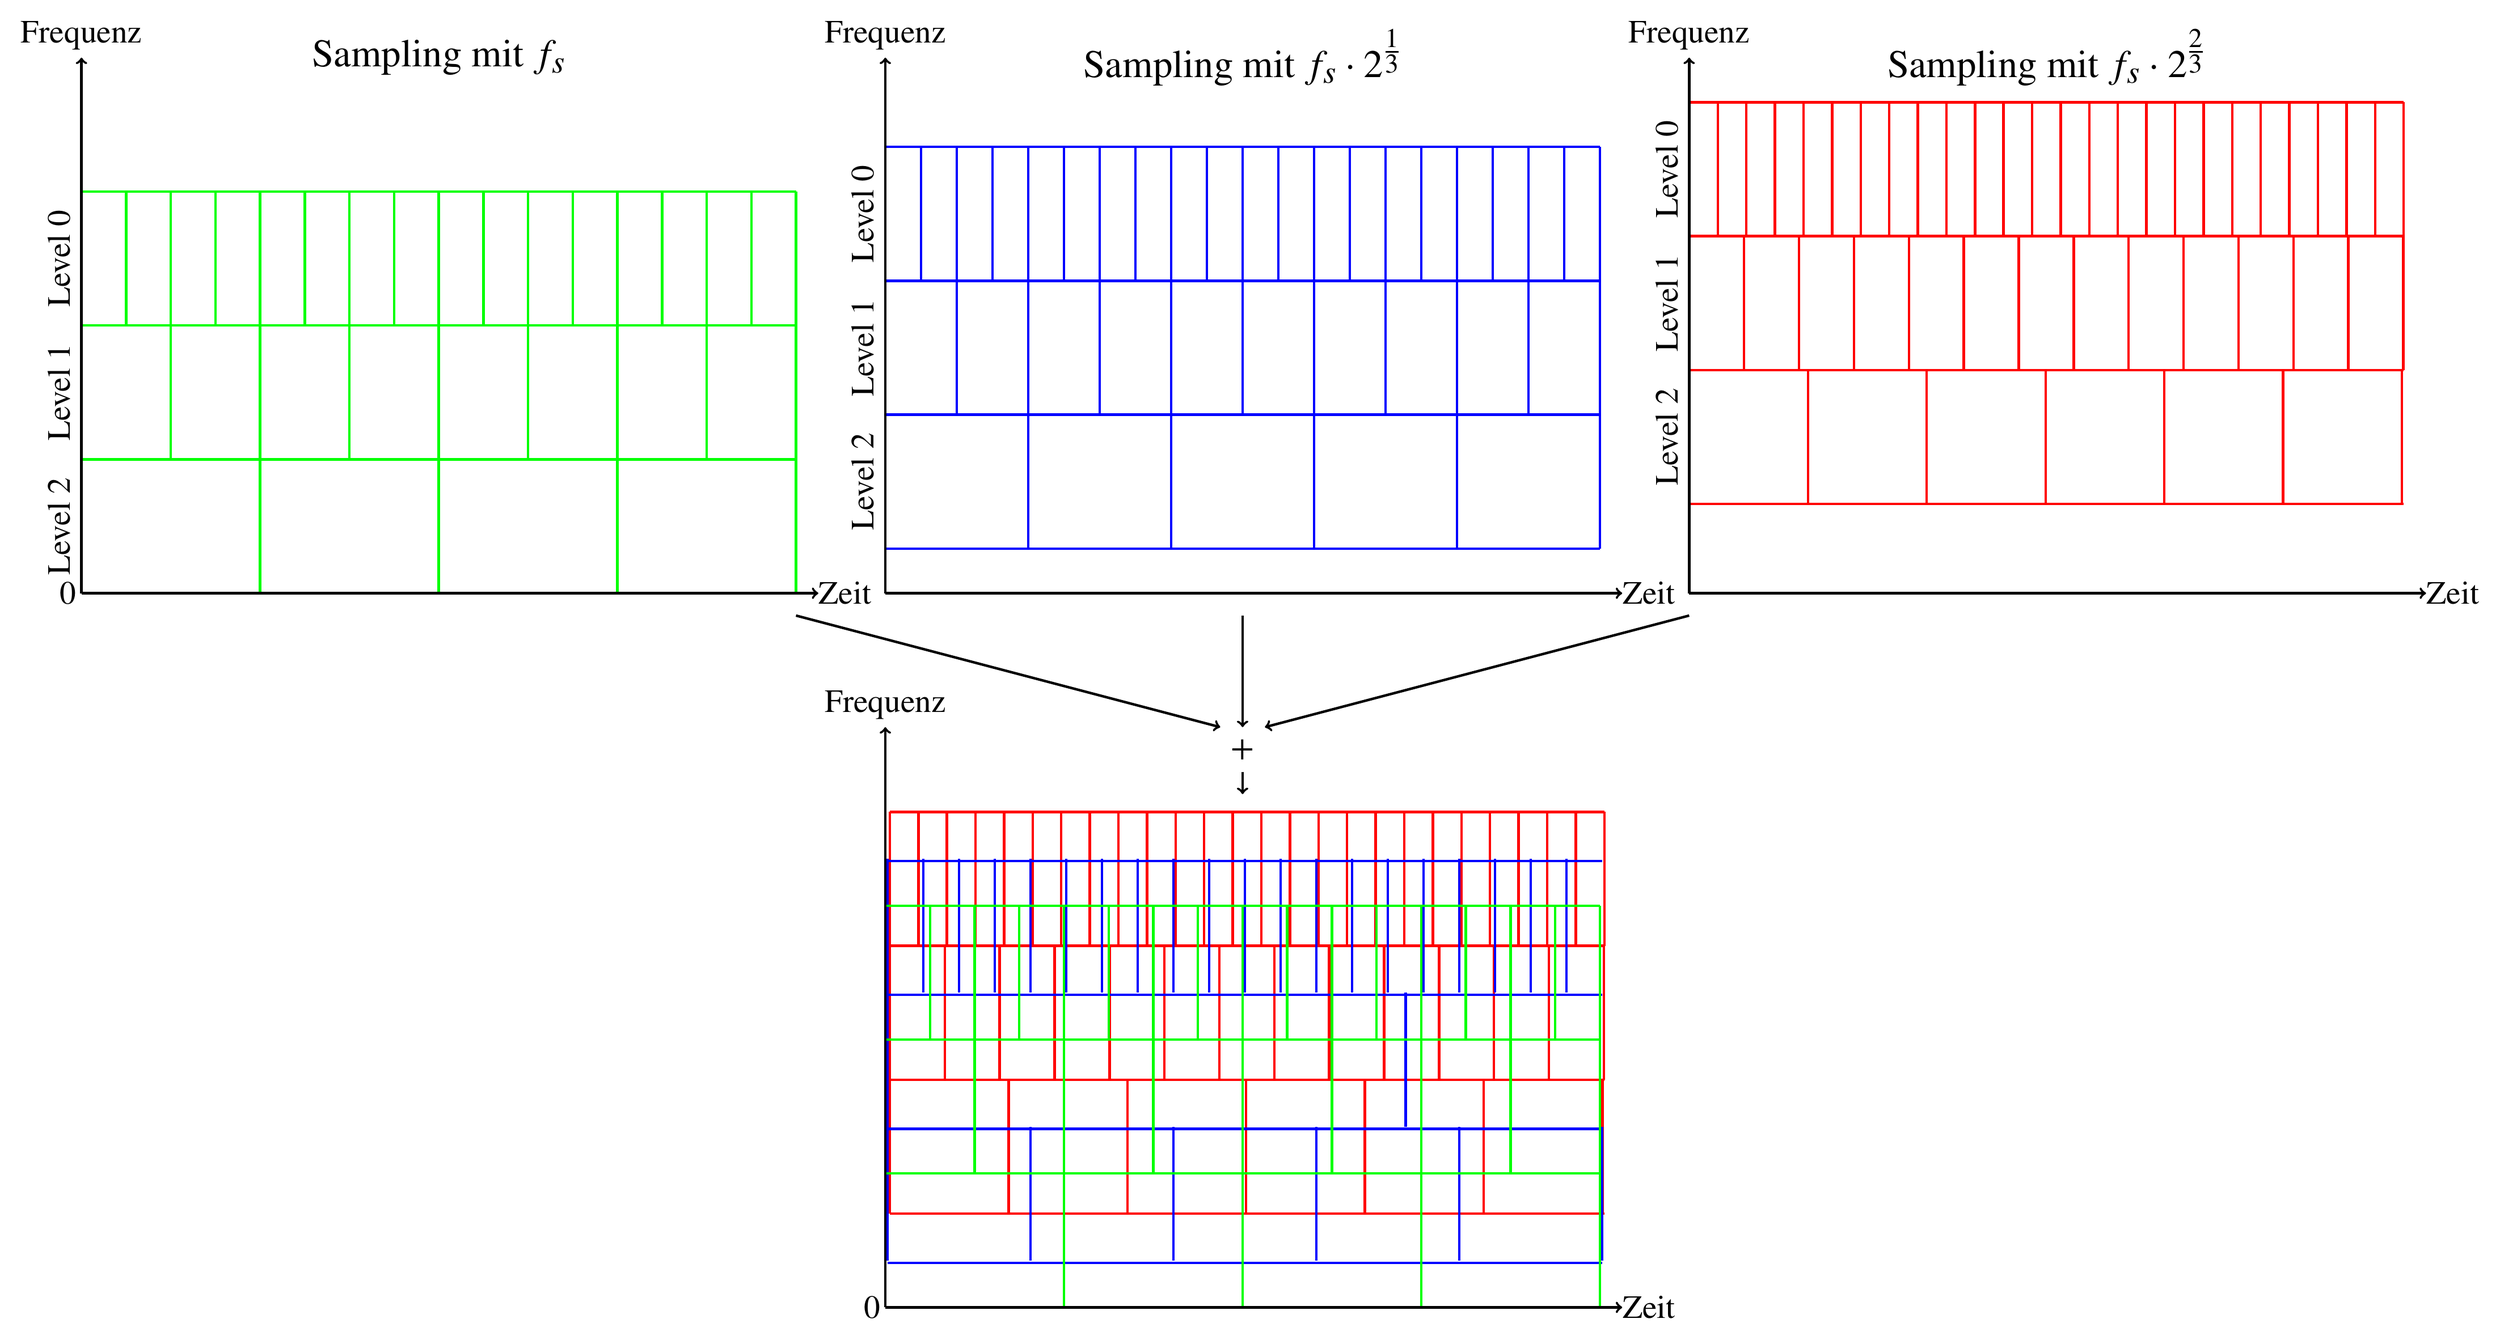
\begin{tikzpicture}






\draw (-0.5,-1.5) node[rotate=90]{\huge Level 0};
\draw (-0.5,-4.5) node[rotate=90]{\huge Level 1};
\draw (-0.5,-7.5) node[rotate=90]{\huge Level 2};

\draw (17.5,-0.5) node[rotate=90]{\huge Level 0};
\draw (17.5,-3.5) node[rotate=90]{\huge Level 1};
\draw (17.5,-6.5) node[rotate=90]{\huge Level 2};

\draw (35.5,0.5) node[rotate=90]{\huge Level 0};
\draw (35.5,-2.5) node[rotate=90]{\huge Level 1};
\draw (35.5,-5.5) node[rotate=90]{\huge Level 2};

\draw (0,3.5) node{\huge Frequenz};
\draw (18,3.5) node{\huge Frequenz};
\draw (36,3.5) node{\huge Frequenz};
\draw (18,-11.5) node{\huge Frequenz};

\draw (8,3) node{\Huge Sampling mit $f_{s}$};
\draw (26,3) node{\Huge Sampling mit $f_{s}\cdot2^{\frac{1}{3}}$};
\draw (44,3) node{\Huge Sampling mit $f_{s}\cdot2^{\frac{2}{3}}$};


\draw (-0.3,-9) node{\huge 0};

\draw (17.7,-25) node{\huge 0};

\draw (17.1,-9) node{\huge Zeit};
\draw (35.1,-9) node{\huge Zeit};
\draw (53.1,-9) node{\huge Zeit};
\draw (35.1,-25) node{\huge Zeit};
\foreach \x in {0,1,...,16}
\draw[ultra thick, green] (\x,0)--(\x,-3);

\foreach \x in {0,2,...,16}
\draw[ultra thick, green] (\x,-3)--(\x,-6);

\foreach \x in {0,4,...,16}
\draw[ultra thick, green] (\x,-6)--(\x,-9);

\foreach \x in {0,-3,...,-9}
\draw[ultra thick, green] (0,\x)--(16,\x);

\draw[ultra thick, ->] (0,-9)--(16.5,-9);
\draw[ultra thick, ->] (0,-9)--(0,3);




\foreach \x in {18,18.8,...,34.1}
\draw[ultra thick, blue] (\x,1)--(\x,-2);

\foreach \x in {18,19.6,...,34.1}
\draw[ultra thick, blue] (\x,-2)--(\x,-5);

\foreach \x in {18,21.2,...,34}
\draw[ultra thick, blue] (\x,-5)--(\x,-8);

\foreach \x in {1,-2,...,-8}
\draw[ultra thick, blue] (18,\x)--(34,\x);

\draw[ultra thick, ->] (18,-9)--(34.5,-9);
\draw[ultra thick, ->] (18,-9)--(18,3);


\foreach \x in {36,36.64,...,52}
\draw[ultra thick, red] (\x,2)--(\x,-1);

\foreach \x in {36,37.23,...,52}
\draw[ultra thick, red] (\x,-1)--(\x,-4);

\foreach \x in {36,38.66,...,52.1}
\draw[ultra thick, red] (\x,-4)--(\x,-7);

\foreach \x in {2,-1,...,-7}
\draw[ultra thick, red] (36,\x)--(52,\x);

\draw[ultra thick, ->] (36,-9)--(52.5,-9);
\draw[ultra thick, ->] (36,-9)--(36,3);



\foreach \x in {18.1,18.74,...,34.1}{
	\draw[ultra thick, red] (\x,-13.9)--(\x,-16.9);
}
\foreach \x in {18.1,19.33,...,34.1}{
	\draw[ultra thick, red] (\x,-16.9)--(\x,-19.9);
}

\foreach \x in {18.1,20.76,...,34.1}{
	\draw[ultra thick, red] (\x,-19.9)--(\x,-22.9);
}
\foreach \x in {-13.9,-16.9,...,-22.9}{
	\draw[ultra thick, red] (18.1,\x)--(34.1,\x);
}


\foreach \x in {18.05,18.85,...,34.05}{
	\draw[ultra thick, blue] (\x,-14.95)--(\x,-17.95);
}
\foreach \x in {18.05,29.65,...,34.05}{
	\draw[ultra thick, blue] (\x,-17.95)--(\x,-20.95);
}

\foreach \x in {18.05,21.25,...,34.05}{
\draw[ultra thick, blue] (\x,-20.95)--(\x,-23.95);
}

\foreach \x in {-15,-18,...,-24}{
	\draw[ultra thick, blue] (18.05,\x)--(34.05,\x);
}


\foreach \x in {18,19,...,34}{
	\draw[ultra thick, green] (\x,-16)--(\x,-19);
}
\foreach \x in {18,20,...,34}{
	\draw[ultra thick, green] (\x,-19)--(\x,-22);
}

\foreach \x in {18,22,...,34}{
	\draw[ultra thick, green] (\x,-22)--(\x,-25);
}
\foreach \x in {-16,-19,...,-25}{
	\draw[ultra thick, green] (18,\x)--(34,\x);
}

\draw[ultra thick, ->] (18,-25)--(34.5,-25);
\draw[ultra thick, ->] (18,-25)--(18,-12);

\draw[ultra thick, ->] (16,-9.5)--(25.5,-12);
\draw[ultra thick, ->] (26,-9.5)--(26,-12);
\draw[ultra thick, ->] (36,-9.5)--(26.5,-12);
\draw (26,-12.5) node[rotate=90]{\Huge +};
\draw[ultra thick, ->] (26,-13)--(26,-13.5);

\end{tikzpicture}

\end{document}

